\subsection{Part Selection}
In our research for part selection we wanted to create a generalized comparison of the options we have available. We formatted this information in the tables below.
\subsubsection{Controller Subsystem}
\begin{flushleft}
	At minimum, any chosen microcontrollers (MCUs) shall support natively, or by addition of a
	module, these features and traits:
	\begin{itemize}
		\item Analog-to-digital converter (ADC)
		\item cURL compatibility
		\item IEEE 802.11
		\item In stock and available to order
		\item JTAG module or equivalent
		\item Module communication bus (UART, I2C, SPI)
		\item Onboard CPU sufficient for our purposes
		\item Onboard memory sufficient for our purposes
		\item Onboard nonvolatile memory
		\item Pins dedicated to analog input
		\item Pins dedicated to digital I/O
	\end{itemize}
	These features would be "nice to have" on any MCU selected, but are not required:
	\begin{itemize}
		\item Digital-to-analog converter (DAC)
		\item microSD card slot
		\item Onboard battery
		\item Pins dedicated to pulse-width modulation (PWM)
		\item Timer(s) and an RTC
		\item USB compatibility
		\item Additional wireless communication protocols (e.g. BT or BLE, Zigbee)
	\end{itemize}
\end{flushleft}
\begin{flushleft}
	The selections, listed in \autoref{table:mcubreakdown1} and not in any particular order, match
	the above criteria and are being considered for selection.
	\begin{table}
		\centering
		\begin{tabularx}{\textwidth}
			{
				| >{\raggedright\arraybackslash}X
				| >{\raggedright\arraybackslash}X
				| >{\raggedright\arraybackslash}X
				| >{\raggedright\arraybackslash}X
				| >{\raggedright\arraybackslash}X
				| >{\raggedright\arraybackslash}X
				|
			}
			\caption{MCU option breakdown}
			\label{table:mcubreakdown1} \\
			\hline
			\textbf{Model} & \textbf{\href{https://www.ti.com/tool/LAUNCHXL-CC26X2R1}{LAUNCH\-XL-CC26X2\-R1}} & \textbf{\href{https://www.ti.com/tool/LAUNCHCC3220MODASF}{LAUNCH\-CC3220\-MODASF}} & \textbf{\href{https://www.raspberrypi.com/products/raspberry-pi-pico/}{Pico W}} & \textbf{\href{https://store-usa.arduino.cc/products/arduino-nano-33-ble?selectedStore=u}{Nano 33 BLE}} & \textbf{\href{https://www.st.com/en/evaluation-tools/b-l4s5i-iot01a.html}{B-L4S5I-IOT01A}} \\
			\hline
			\textbf{Manu\-facturer} & Texas Instruments & Texas Instruments & Raspberry Pi & Arduino & STMicro\-electronics \\
			\hline
			\textbf{Micro\-controller} & CC2652R & CC3220\-MODASF & RP2040 & nRF52840 & STM32\-L4S5VIT6 \\
			\hline
			\textbf{Processor} & 1x ARM Cortex-M4F & 1x ARM Cortex-M4 & 2x ARM Cortex-M0+ & 1x ARM Cortex-M4 & 1x ARM Cortex-M4 \\
			\hline
			\textbf{Maximum Speed (MHz)} & 48 & 80 & 133 & 64 & 120 \\
			\hline
			\textbf{Memory (KB)} & 256 ROM, 352 flash, 100 SRAM & 1024 flash, 256 RAM & 16 ROM, 264 SRAM & 1024 flash, 256 SRAM & 2048 flash, 640 RAM \\
			\hline
			\textbf{Wireless capability} & BLE5.2, Zigbee, Thread & 802.11b/g/n & 802.11n & BLE5.3, Zigbee, Thread, Matter & BT4.1, 802.11b/g/n, NFC \\
			\hline
			\textbf{Serial capability} & UART, I2C, I2S, SPI & UART, I2C, SPI & UART, I2C, SPI, USB1.1 & UART, I2C, I2S, SPI, USB2.0 & UART, I2C, SPI, USB2.0 \\
			\hline
			\textbf{Price (\$)} & 40, maybe free & 60, maybe free & 6 & 28 & 53 \\
			\hline
			\textbf{ADC} & 8-channel, 12-bit & 4-channel, 12-bit & 4-channel, 12-bit & 8-channel, 12-bit & 16-channel, 12-bit \\
			\hline
			\textbf{Clock capability} & Timer, RTC & Timer, RTC, WDT & Timer, RTC, WDT & Timer, RTC, WDT & Timer, RTC, WDT \\
			\hline
			\textbf{GPIO (pins)} & 31 & 29 & 30 & 13 & 16 \\
			\hline
			\textbf{PWM (channels)} & Supported & Supported & 16 & 4 & 6 \\
			\hline
			% \textbf{AES (bits)} & 128, 256 & 256 & Not supported & 128 & 128 \\
			% \hline
			\textbf{Required voltage (V)} & 1.8 -- 3.8 & 2.3 -- 3.6 & 1.8 -- 3.3 & 4.5 -- 21 & 4.75 -- 5.25 \\
			\hline
		\end{tabularx}
	\end{table}
\end{flushleft}
\begin{flushleft}
	Use of single-board computers (SBCs) was considered, but will not not need to be used; cURL 
	used on an MCU in conjunction with \href{https://aws.amazon.com/ec2/}{Amazon EC2} services will
	allow us to offload computing to a cloud solution.
\end{flushleft}
\begin{flushleft}
	Use of an external Wifi module is discouraged due to the following:
	\begin{itemize}
		\item Added cost
		\item Added complexity
		\item Modules in common use by hobbyists often have poor or no proper documentation, to the
		extent of:
		\begin{itemize}
			\item Quick start guide
			\item User's guide
			\item Datasheets
			\item Theory of operation
			\item Application uses
			\item Troubleshooting guide
			\item Schematics and mechanicals
			\item Quality and reliability
			\item Errata
		\end{itemize}
	\end{itemize}
\end{flushleft}
\begin{flushleft}
	Therefore, all of the MCUs listed above support either the 802.11 or Bluetooth standards.
\end{flushleft}
\begin{flushleft}
	Ultimately, the \href{https://www.ti.com/tool/LAUNCHCC3220MODASF}{LAUNCHCC3220MODASF}
	was chosen as the microcontroller development board for this project. In the event that the
	aforementioned LaunchPad is not able to be obtained, the
	\href{https://www.ti.com/tool/CC3220SF-LAUNCHXL}{CC3220SF-LAUNCHXL} has equivalent capability
	for the project's needs.
\end{flushleft}
\begin{flushleft}
	These boards, henceforth referred to as the CC3220, are able to be requested from our
	university at no upfront cost to our team. This was the driving factor behind choosing 
	the CC3220 over other microcontroller development boards. It was also determined that
	the microcontroller \emph{must} be able to interface via the 802.11 (WiFi) standard, for reasons
	that are detailed in \autoref{sec:controller_subsystem}---therefore, the LAUNCHXL-CC26X2R1
	and Nano 33 BLE were disqualified from selection. The Pico W was considered due to its low cost,
	and the B-L4S5I-IOT01A considered because of its abundant peripherals, but both ultimately lost
	out to the Texas Instruments products.
\end{flushleft}
% End Controller Subsystem

\subsubsection{Power Subsystem}
\paragraph{Power Supply}
The power system is a key factor to this model and trying to make this an independent system. This is key because this power system needs to be able to power all of the many different components, while also charging itself when not operating.

As part of the goal to make this an independent system, solar energy plays a great role in this and making this system run. Before anything as well, this part of the system must operate first before it can power other components. For this system to run, the key parts include: solar panels that convert light energy into electrical energy; solar charge controller to regulate output voltage from the solar panel into the battery; the battery to directly power the other components in the model.

In this model there are many different sensors, electrical, and mechanical components all of which require power. This requires a design of how the power system will flow and operate. It first begins with determining the total power needed for the whole system to run. This can be determined by finding the individual power ratings of each component and calculating them all together. After that is found, we can then choose what type of battery and the quantity needed for the model. When choosing what kind of battery and how many is needed, how long we want the system to run, optional secondary power source, and optional battery bank must be put into consideration as well. As follows, we begin to research solar panels from type, efficiency, power rating, etc. Then, a solar charge controller must be selected, a device that sits between the solar panel and the battery to regulate how much power is going into the battery. Once that is done, a voltage regulator must be determined, to regulate voltage from the battery to the smaller components that need to be powered. After all that is done, then we can find other components that will make the power system more reliable and efficient in any way.

\paragraph{Power Requirement}
Sensors, electrical, and mechanical components all require power but all consume different amounts of power. As mentioned before, analyzing the total power requirement is important and crucial because this will help us determine the right parts that will be best for this system and for the components.

With the total power determined, the Watts per hour needed for all of the components to run must also be found. The watts per hour is important too because this helps figure out how long each component will operate for. After that is found, we used the altE calculator to help pick out what kind of battery can be used, then solar panel and solar charge controller, respectively. The altE calculator is a great resource because with the proper measurements, it can help us choose what kind of battery we can use, by determining the capacity needed in watt-hours or amp-hours. This calculator can also help us choose how big of a solar panel we need and how big of a solar charge controller we need as well.
\paragraph{Rechargeable Battery Selection}
Solely relying on solar energy isn’t always ideal. This is because the weather may not always guarantee sunlight, this will hinder its power retention. For this reason, solar panels are paired with a battery so that the power can be stored and then used at a later time. As part of the goal to have this run as an independent system, an additional battery may be used so that one battery can power the system while the other one can charge.

There are many different types of batteries including Nickel-Cadmium, Nickel-Metal Hydride, Lithium ion, etc. Of the three batteries, they will be compared to see which will best fit our model and which will fulfill the requirements on the basis of power output, efficiency, etc.

Nickel Cadmium (NiCd) batteries in today’s time are used for RC vehicles, power tools, photography equipment, and more. They would also be considered as old technology. Even though they are old, they still have their advantages such as being less expensive, they are super powerful and charge fast, they require little maintenance, and more. These batteries though also has its disadvantages, one being they suffer from “ memory” problems and as a result of that, it may reduce that capacity of charges and future battery life. These batteries are also environmentally concerning because cadmium is toxic.

Nickel-Metal Hydride (NiMH) is similar to nickel cadmium, the only difference is that hydrogen is used instead of cadmium as the active element. Hybrid cars, toothbrushes, and phones are just a few of many products that use nickel-metal hydride batteries and have been used in these appliances because of the trouble free service they grant. It is also because even being partially discharged, it can be charged as many times and will always be at full capacity. Even with advantages like that nickel-metal hydride batteries produce a lot of heat when in use, have a high self-discharge rate, and have memory issues as well, just not as bad as NiCd.

Lithium ion batteries, one of the most popular types of rechargeable batteries for portable products. It is considered the best because lithium ion batteries have high open circuit voltage, low self-discharge rates, and little to no memory effect. On top of that they are growing within the military, electric vehicle companies, and aerospace industry with little to no maintenance. Even though they have a lot of advantages, some of the disadvantages include sensitivity towards high temperatures, it cannot be fully discharged, and the cost.

Through much consideration and investigation, the four batteries listed in the following table were picked. All of which are 12V lithium iron phosphate (LiFePO4) batteries. Then the selected battery that we decided we were going to use for this model is the Eco Worthy 12V 8Ah LiFePO4 battery. We decided to go with this battery because although it is a little expensive,the Watts per hour and the Ah rating that this battery provides, was great for what we plan on having.

\begin{table}[H]
    \centering
	
	\begin{tabularx}{\textwidth}
		{
			| >{\raggedright\arraybackslash}X
			| >{\raggedright\arraybackslash}X
			| >{\raggedright\arraybackslash}X
			| >{\raggedright\arraybackslash}X
			| >{\raggedright\arraybackslash}X
			|
		}
		\caption{Battery Selection}
		\label{table:rechargeablebatteryl} \\
		\hline
		\textbf{Manu\-facturer} & \textbf{Ampere Time} & \textbf{Eco Worthy} & \textbf{Expert\-Power} & \textbf{Eco Worthy} \\
		\hline
		\textbf{Voltage} &  12 & 12 & 12 & 12 \\
		\hline
		\textbf{mAh} &  6000 & 10000 & 5000 & 8000 \\
		\hline
		\textbf{Watt per hour} & 76.8 & 120 & 64 & 96 \\
		\hline
		\textbf{Cost} & \$29.99 & \$59.99 & \$35.99 & \$43.99 \\
		\hline
	\end{tabularx}
\end{table}
\paragraph{Solar Panel Selection}
Solar has been a growing source of energy in the past years, with new developments and breakthroughs with solar cell technology. As the whole purpose of solar energy is to collect sunlight and convert it into electrical energy, that is the minimum for this model to run as an independent system. Then as a stretch goal, we would apply the concept of solar tracking panels to create blinds with the solar panels so it can open and close according to the position of the sun.

On a basic level, solar panels are made of solar cells and these cells do the collecting and converting. These solar cells are made from crystalline silicon that is melted down into ingots and then cut into sheets. In the solar industry there are 3 main types of solar panels. These types of panels are monocrystalline, polycrystalline, and thin-film panels all of which have different compositions. Each type has different efficiencies, generating different amounts of power, etc.

Monocrystalline solar panels are solar panels that are made with monocrystalline solar cells. These solar cells are composed of a single silicon crystal which provides electrons more space to move because of the electricity flow that is generated. This makes them more efficient, yet at the same time more costly. Polycrystalline solar panels are solar panels that are made with polycrystalline solar cells. Similar to monocrystalline solar cells, they are made of a silicon crystal, the only difference is that instead of a single crystal, they use several fragments of silicon to form an ingot and that is cut into sheets. As a result of melting several fragments into one it creates a mosaic look as well as giving it a blue hue, whereas the monocrystalline solar panel will have a uniform color and look. Aesthetically, they might look nicer but they are less efficient than monocrystalline solar panels. This also means that they aren’t going to be as pricey compared to the monocrystalline panels because of the efficiency and manufacturing process. Thin-film solar panels differ from crystalline solar panels greatly, all because they are made with different materials. The three main types of thin-film solar panels are amorphous silicon (a-Si), cadmium telluride (CdTe), and copper indium gallium selenide (CIGS). Currently, thin-film solar panels are the least efficient, costly, and have the shortest lifespan. It is predicted that they will have a major growth in the solar industry because although they are the least efficient, they have a higher theoretical efficiency than both monocrystalline and polycrystalline.

The choice of solar panels will be based on multiple aspects of each type of solar panel. As we know, the efficiency rating and cost from most to least will go from monocrystalline, polycrystalline, and thin-film, respectively, but we must also look at its temperature coefficient, power rating, and more to be able to determine which solar panel we exactly need. Temperature coefficient for solar panels is the power lost as the temperature rises. This plays a very important role because we live in Florida, temperatures can get hot. So, when it comes to which solar panel will still be more efficient in higher temperatures, monocrystalline solar panels are still the best. As follows, it then goes from polycrystalline and then thin-film. This doesn’t mean we shouldn’t count them out though, because depending on where you live the temperatures may not be high so it won’t impact it as much. It could also be more cost efficient as well because the other two types of solar panels are less expensive. Another factor to keep in mind is the power capacity of each solar panel type. For monocrystalline solar panels, because of their single crystal structure it allows for a higher power output, compared to polycrystalline, its power output capacity isn’t as high. For thin-film panels, because they don’t have uniform sizes, they won’t have a standard for power capacity.


\begin{table}[H]
    \centering
	
	\begin{tabularx}{\textwidth}
		{
			| >{\raggedright\arraybackslash}X
			| >{\raggedright\arraybackslash}X
			| >{\raggedright\arraybackslash}X
			| >{\raggedright\arraybackslash}X
			|
		}
		\caption{Solar panel types}
		\label{table:solarpanel} \\
		\hline
		\textbf{Solar Panel Type} & \textbf{Mono\-crystalline} & \textbf{Poly\-crystalline} & \textbf{Thin - Film} \\
		\hline
		\textbf{Efficiency} &  \textgreater20\% & 15 - 17\% & 6 - 15\% \\
		\hline
		\textbf{Power Rating} &  $\le$300W & 240 - 300W & Indefinite \\
		\hline
		\textbf{Performance} & Most efficient & Efficient & Least efficient \\
		\hline
		\textbf{Temperature} & High Tolerance & Low Tolerance & High Tolerance \\
		\hline
		\textbf{Cost per Watt} & \$1 - \$1.50 & \$.70 - \$1 & \$.43 - \$.70 \\
		\hline
	\end{tabularx}
\end{table}
Through research and investigation, different solar panels were compared to see which would be best fit for our model. With the different types of solar panels, we didn’t specifically choose what kind of solar panel type we wanted to go with because they all were great options and benefited in various ways. Of the four choices listed in the following table though, the monocrystalline solar panel was a popular type. These solar panel choices that were picked, all have a power rating of 10 Watts and a voltage rating of 12V, except for the Voltaic solar panel which was 18V. \par
The selected solar panel that we chose was the Eco Worthy 10W 12V monocrystalline. There were a lot of factors that went into this choice, one of them was because of the cost of the solar panel, it was a great price for what we were getting. It was also because of the size and weight, it makes it very easy to move around. Also, it had many great reviews and is available on different websites to order.\par
\begin{table}[H]
    \centering
	\caption{Solar panel part breakdown}
	\label{table:solarpanelparts}
	\begin{tabularx}{\textwidth}
		{
			| >{\raggedright\arraybackslash}X
			| >{\raggedright\arraybackslash}X
			| >{\raggedright\arraybackslash}X
			| >{\raggedright\arraybackslash}X
			| >{\raggedright\arraybackslash}X
			|
		}
		\hline
		\textbf{Sku} & P108 & L02M10-1 & NPA10S-12H & SLP010-12U \\
		\hline
		\textbf{Manu\-facturer} & \textbf{Voltaic Systems} & \textbf{Eco Worthy} & \textbf{Newpowa} & \textbf{SolarLand} \\
		\hline
		\textbf{Solar Panel Type} & Monocrystalline & Monocrystalline & Monocrystalline & Polycrystalline \\
		\textbf{Dim\-ensions} & 10.9 x 8.8 x .16 & 13.3 x 8.1 x .7 & 14.37 x 7.68 x .91 & 14.06 x 11.89 x 1.18 \\
		\hline
		\textbf{Peak Current} & 570mA & 580mA & 630mA & 580mA \\ 
		\hline
		\textbf{Open Circuit Voltage} & 20.45V & 20.6V & 19.83V & 21.6V \\
		\hline
		\textbf{Peak Voltage} & 17.34V & 17.3V & 16.77V & 17V \\
		\hline
		\textbf{Wattage} & 9 watt & 10 watt & 10 watt & 10 watt \\
		\hline
		\textbf{Power Tolerance} & $\pm$10\% & $\pm$3\% & $\pm$3\% & $\pm$5\% \\
		\hline
		\textbf{Cost} & \$49 & \$25.99 & \$25.99 & \$35.53 \\
		\hline
	\end{tabularx}
\end{table}
\paragraph{Solar Charge Controller Selection}
Solar charge controllers play an important role in this system because this system is running on solar energy. A solar charge controller is a regulator that goes in between the solar panel and the battery, regulating the total output power coming out of the solar panel. This is important because this will prevent the battery from overcharging and possibly reducing its effectiveness. If the wrong charge controller was picked, it could result in a loss of power that is generated, and can harm any device. As stated in the power requirement section, finding the total power needed for the whole system is important because we can use that to help determine the proper charge controller to get. \par
There are two main types of solar charge controllers: Maximum Power Point Tracking (MPPT) and Pulse Width Modulated (PWM). Choosing the right charge controller is based on current and voltage characteristics. This is because they regulate input voltage coming in from the solar panel and output voltage of what is coming out to the battery.\par
Maximum power point tracking (MPPT) is a technique that observes and regulates energy coming from the solar panel and into the battery. What makes this special is that it can match the solar panel voltage to the battery voltage, which allows it to maximize the charge efficiency. They operate as a DC to DC converter, taking in high DC input from the solar panel, changing it to high AC voltage, then back down to DC voltage.\par
Pulse width modulated (PWM) solar charge controllers are considered the original charge controller compared to the MPPT charge controller. They are less expensive and the technique behind this controller is also simpler. On a basic level, the PWM controller acts as an on-off regulator. When the battery voltage reaches a certain level, the PWM controller will slowly reduce the charging current, up until the battery reaches the maximum amount of energy. This makes it great for smaller installations because the solar panel and the controller can match better. \par
While looking at different solar charge controllers, we came across 4 different controllers, all of which are PWM charge controllers. We did not specifically choose the PWM controller but through our search for what charge controller we wanted to use all of the choices we found were PWM. This would be great for our model regardless because our system will not be large and it will be less expensive compared to MPPT charge controllers.\par
The solar charge controller we chose for our model is the Eco Worthy 10A PWM solar charge controller. The reason we chose this controller is because it comes as a kit along with the solar panel. As a result of it coming as a kit with the solar panel they will already be very compatible together and the price for both of them together is not expensive at all. \par
\begin{table}[H]
    \centering
	\begin{tabularx}{\textwidth}
			{
			| >{\raggedright\arraybackslash}X
			| >{\raggedright\arraybackslash}X
			| >{\raggedright\arraybackslash}X
			| >{\raggedright\arraybackslash}X
			| >{\raggedright\arraybackslash}X
			|
		}
		\caption{Charge Controller}
		\label{table:chargecontroller} \\
		\hline
		\textbf{Manu\-facturer} & \textbf{Eco Worthy} & \textbf{Renogy} & \textbf{Expert\-Power} &  \textbf{Expert\-Power} \\
		\hline
		\textbf{Charge\-Controller Type} & PWM & PWM & PWM & PWM \\
		\textbf{Output Voltage} & 12\slash24V  & 12\slash24V & 12\slash24V & 12\slash24V \\
		\hline
		\textbf{Rated Charge Current} & 10A & 10A & 10A & 20A \\
		\hline
		\textbf{Max PV Voltage} & 30V & 50V & 55V & 55V \\
		\hline
		\textbf{Self Consumption} & $\leq$10mA & $\leq$10mA & \textless10mA & $\leq$13mA \\
		\hline
		\textbf{Price (\$)} & 23.99 & 69.99 & 34.99 & 69.99 \\ 
		\hline
	\end{tabularx}
\end{table}
While the model is charging during the day or as a back up, this will be plugged into a wall outlet for power. This means we have to be able to convert the AC voltage coming from the wall is converted to DC voltage for the model to use.
\begin{table}[H]
    \centering
	\begin{tabularx}{.8\textwidth}
		{
			| >{\raggedright\arraybackslash}X
			| >{\raggedright\arraybackslash}X
			| >{\raggedright\arraybackslash}X
			| >{\raggedright\arraybackslash}X
			|
		}
		\caption{AC/DC Converter breakdown}
		\label{table:acdcconverter} \\
		\hline
		\textbf{Manu\-facturer} & \textbf{SmoTecQ} & \textbf{ANLINK} & \textbf{TMEZON} \\
		\hline
		\textbf{Input Voltage} &  240V & 100 - 240V & 100 - 240V \\
		\hline
		\textbf{Output Voltage} & 12V & 12V & 12V \\
		\hline
		\textbf{Current Rating} & 2A & 2A & 2A \\
		\hline
		\textbf{Connector} &  5.5 mm x 2.1 mm &  5.5 mm x 2.1 mm &  5.5 mm x 2.1 mm\\
		\hline
		\textbf{Price (\$)} & 12.99 for 2 & 11.59 & 8.99 \\ 
		\hline
	\end{tabularx}
\end{table}

\subsubsection{Sensing Subsystem}
The required sensing subsystem capabilities include:
    \begin{itemize}
        \item Spectral frequency separation
        \item Spectral range from 400 to 1700nm
        \item High Signal to Noise Ratio
    \end{itemize}


	Silicon photodiodes have a spectral range across the visible spectrum, usually spanning from 350 to 1000nm. In order to generate spectrographs with the relevant molecular fingerprints of soil substances, we're going to need an infrared detector. InGaAs stands out as the ideal material for this range, with most sensors ranging from 800 to 1700nm. There are several manufacturers of silicon photodiodes, and most of them offer a small selection of InGaAs photodiodes at low prices as well. Below are the four of each.


\begin{table}[H]
	\centering
	\label{table:VISsensors}
	\caption{VIS Sensors}
	\begin{tabular}{|p{2cm}|l|l|l|l|}
	\hline    
	Model & BPX 61 & ODD-5W & FDS100 & PIN-3CD\\
    \hline
	Manufacturer & Newark & Digikey Opto Diode Corp & Thorlabs & Edmund Optics\\
    \hline
	Spectral Range (nm) & 400-1100 & 300-1100 & 350-1100 & 350-1100\\
    \hline
	Active Area (mm sqrd) & 7.02 & 5 & 13 & 3.2\\
    \hline
	Cost (\$) & 13.06 & 14.50 & 16.08 & 34.00\\
    \hline
	\end{tabular}
\end{table}



\begin{table}[H]
	\centering
	\label{table:NIRsensors}
	\caption{NIR Sensors}
	\begin{tabular}{|p{2cm}|l|l|l|l|}
	\hline    
	Model & C30617BH & 0800-3111-011 & FGA015 & N/A\\
	\hline
	Manufacturer & Digikey Excelitas & Digikey Advanced Photonix & Thorlabs & Edmund Optics\\
	\hline
	Spectral Range (nm) & 800-1700 & 800-1700 & 800-1700 & 800-1700\\
	\hline
	Active Area (mm sqrd) & 0.1 & 1.36 & 0.018 & 0.12\\
	\hline
	Cost (\textdollar) & 43.58 & 50.21 & 63.00 & 88.00 \\
	\hline
	\end{tabular}
\end{table}


From the above, we selected the Newark BPX 61 for our Silicon photodiode and the Excelitas C30617BH for our InGaAs photodiode.

Here are the spectral sensitivity curves for each:

\begin{figure}[H]
    \caption{VIS Photodiode Spectral Sensitivity}
    \centering
    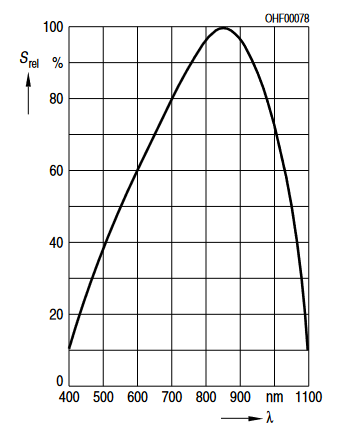
\includegraphics[width=\textwidth]{images/NewarkBPX61.png}
\end{figure}

\begin{figure}[H]
    \caption{NIR Photodiode Spectral Sensitivity}
    \centering
    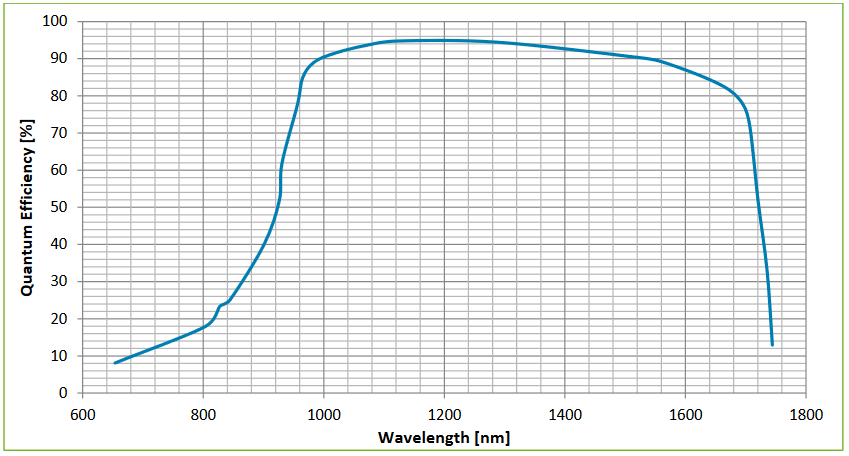
\includegraphics[width=\textwidth]{images/DigikeyExcilitasNIRSensor.png}
\end{figure}